\documentclass[a4paper,12pt,table]{exam}
\usepackage{pacote_provas_guizao}
\newcommand{\data}{19/11/2024}
\newcommand{\professor}{Guilherme Schultz Netto}
\newcommand{\valor}{4,0}
\newcommand{\serie}{2\textsuperscript{a} SÉRIE}
\newcommand{\media}{2,8}
\newcommand{\aluno}{completo}
\begin{document}
\begin{center}
    \begin{table}
        \centering
        \begin{tabular}{|>{\raggedright\arraybackslash}p{0.2\linewidth}|>{\raggedright\arraybackslash}p{0.2\linewidth}|>{\raggedright\arraybackslash}p{0.2\linewidth}|>{\raggedright\arraybackslash}p{0.2\linewidth}|} \hline  
             \multicolumn{4}{|l|}{\LARGE\textbf{AVALIAÇÃO SOMATIVA DE MATEMATICA} \hspace{1 cm}
\includegraphics[scale=0.9]{logomarista.jpg}} \\ 
             \multicolumn{4}{|l|}{\Large\textit{3\textsuperscript{o} TRIMESTRE}} \\ \hline  
             \multicolumn{3}{|l|}{\textbf{ALUNO(A): completo}}& \textbf{SÉRIE/ANO:\serie}\\ \hline  
             \multicolumn{3}{|l|}{\textbf{PROFESSOR: \professor}}& \textbf{TURMA: A}\\ \hline  
            \textbf{VALOR:\valor}&  \textbf{MÉDIA:\media}&  \textbf{NOTA:}& \textbf{DATA:\data}\\ \hline  
             \multicolumn{4}{|l|}{\textbf{ASSINATURA DO RESPONSAVEL:}}\\ \hline  
             \multicolumn{2}{|c|}{
\noindent\begin{minipage}[t]{0.48\linewidth}%
  Querido estudante, leia atentamente as recomendações:
  \fullwidth{
  \begin{description}[ align=left, leftmargin=*]
  \item[\textbullet] A prova deve ser feita à tinta azul ou preta.
      \item[\textbullet] Não é permitido usar corretivo.
      \item[\textbullet] A questão objetiva que apresentar rasura será anulada.
      \item[\textbullet] Letra legível e organização são fundamentais para a correção das questões.
      \item[\textbullet] Dê respostas completas e bem estruturadas para que não se sinta prejudicado(a) posteriormente.
      \item[\textbullet] A interpretação das questões faz parte da avaliação. Lembre-se que \textbf{você será avaliado pelo que escreveu e não pelo que pensou em escrever.}
      \item[\textbullet] \textbf{Todas as questões devem conter os cálculos para justificar sua resposta.}
      \item[\textbullet] Não use ``meios inadequados" para a realização da prova (comunicar-se com colegas, ``colar" ou portar ``cola"). Caso haja algumas dessas ações, ocorrerá, para os envolvidos, a anulação das provas, sem direito à 2\textsuperscript{a} chamada.
      \begin{flushright}
          Boa Prova!
      \end{flushright}
  \end{description}
  }
\end{minipage}}&  \multicolumn{2}{|c|}{
\noindent\begin{minipage}[t]{0.48\linewidth}%
  \textbf{\textit{HABILIDADES:}}
  \vspace{0.1 cm}
  \fullwidth{
  \begin{description}[align=left, leftmargin=*]
    \item[\textbullet] H2: Identificar padrões numéricos ou princípios de contagem.
    \item[\textbullet] H3: Resolver situação-problema envolvendo
conhecimentos numéricos.
\item[\textbullet] H5: Avaliar propostas de intervenção na realidade
utilizando conhecimentos numéricos.
\item[\textbullet] H7: Identificar as características de figuras planas ou
espaciais.
\item[\textbullet] H8: Resolver situação-problema que envolva
conhecimentos geométricos de espaço e forma.
\item[\textbullet] H9: Utilizar conhecimentos de espaço e forma na
seleção de argumentos propostos como solução de
problemas do cotidiano.
\item[\textbullet] H10: Identificar relações entre grandezas e unidades de
medida.
\item[\textbullet] H15: Identificar a relação de dependência entre
grandezas.
\item[\textbullet] H19: Identificar representações algébricas que
expressem a relação entre grandezas.
  \end{description}
  }
\end{minipage}}\\ \hline 
        \end{tabular}
    \end{table}
\end{center}
\begin{questions}
\fullwidth{\question[0,4] O laboratório de insetos da UFES contem besouros (com 6 pernas cada) e aranhas (com 8 pernas cada). O número total de pernas excede em $214$ o número de aranhas e besouros. O número de aranhas é inferior em 14 ao número de besouros. Calcule e assinale corretamente o número de aranhas.
\begin{randomizechoices}
\choice $15$.
\choice $14$.
\choice $13$.
\choice $12$.
\choice $11$.
\end{randomizechoices}

}
\newpage
\fullwidth{\question[0,4] É importante saber como os computadores representam e processam dados. Sabendo que os computadores utilizam o sistema binário para representar informações, assinale a alternativa que explica corretamente o motivo dessa escolha.

\begin{randomizechoices}
\choice Porque o sistema binário é o mais simples para os humanos entenderem e utilizarem na programação.
\CorrectChoice Porque os computadores operam com componentes eletrônicos que têm dois estados estáveis, representando 0 e 1, o que torna o sistema binário adequado.
\choice Porque o sistema binário permite representar números negativos sem a necessidade de complementos.
\choice Porque o sistema binário ocupa menos espaço de armazenamento em comparação com outros sistemas numéricos.
\choice Porque o sistema binário foi escolhido arbitrariamente pelos primeiros programadores e se tornou padrão.
\end{randomizechoices}
}
\fullwidth{\question[0,4] 
Durante uma aula de Computação, o professor Guilherme abordou os conceitos fundamentais de algoritmos. Ele explica que um algoritmo é uma sequência finita de instruções bem definidas que resolve um problema específico. Entre as características essenciais de um algoritmo, assinale qual das alternativas abaixo está incorreta.

\begin{randomizechoices}
\choice Um algoritmo deve ser composto por passos finitos e bem definidos.
\choice Um algoritmo pode ter zero ou mais entradas.
\CorrectChoice Um algoritmo deve ser escrito em uma linguagem de programação específica, como Python ou Java.
\choice Um algoritmo deve produzir pelo menos uma saída.
\choice As instruções de um algoritmo devem ser efetivas, executáveis em tempo finito.
\end{randomizechoices}

}
\fullwidth{\question[0,4]

Em uma atividade prática, os alunos estão aprendendo a criar algoritmos em pseudocódigo. O professor apresenta o seguinte algoritmo:

\begin{center}
        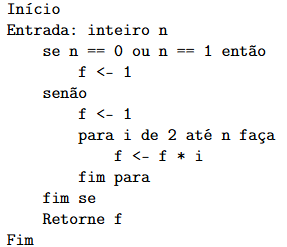
\includegraphics[width=0.3\linewidth]{codigo.png}
\end{center}

Júlia executou o algoritmo com \( n = y \) e obteve como retorno \( 120 \). Determine o valor de $y$ escolhido por Júlia.

\begin{randomizechoices}
\CorrectChoice \( y = 5 \).
\choice \( y = 6 \).
\choice \( y = 4 \).
\choice \( y = 7 \).
\choice \( y = 10 \).
\end{randomizechoices}

}
\newpage
\fullwidth{\question[0,4] Durante a aula de Computação, o professor Guilherme explicou a diferença entre software e hardware, bem como entre linguagens de programação de alto nível e baixo nível. Ele afirmou que a compreensão dessas diferenças é fundamental para entender como os programas são executados em um computador.

Assinale, dentre as afirmações abaixo, a que está CORRETA em relação a linguagens de programação e sua relação com hardware e software.

\begin{randomizechoices}
\choice Linguagens de baixo nível, como Python e Java, são independentes de hardware e mais próximas da linguagem humana.
\CorrectChoice Linguagens de alto nível, como Python e Java, são independentes de hardware e mais próximas da linguagem humana.
\choice Linguagens de alto nível são diretamente executadas pelo hardware sem necessidade de tradução.
\choice Linguagens de baixo nível não requerem conhecimento detalhado do hardware para programação eficiente.
\choice Linguagens de alto nível fornecem controle direto sobre registradores e memória, permitindo programação de sistemas operacionais.
\end{randomizechoices}}
\fullwidth{\question[0,4] 
Existe uma diferença natural entre Hardware e Software, como discutido. Assinale a alternativa que contém, das afirmações abaixo, a que descreve corretamente essa diferença.

\begin{randomizechoices}
\choice Hardware refere-se aos programas e aplicativos que executam tarefas específicas, enquanto software é o conjunto de componentes físicos do computador.
\CorrectChoice Hardware são os componentes físicos de um computador, como CPU e memória, enquanto software é o conjunto de instruções que comandam o hardware.
\choice Hardware e software são termos intercambiáveis que ambos se referem aos componentes físicos de um sistema de computação.
\choice Software é qualquer dispositivo de entrada ou saída, enquanto hardware são os dados processados pelo computador.
\choice Hardware é o sistema operacional do computador, enquanto software são os componentes eletrônicos internos.
\end{randomizechoices}
}
\fullwidth{\question[0,4] Uma das utilizações dos determinantes é a possibilidade de verificar a existência (ou a finitude) de soluções para um sistema linear. Faça o que é pedido:
\begin{enumerate}[label=\Alph*)]
    \item Determine o valor do parâmetro $\Psi$ para que o seguinte sistema a seguir tenha solução única:
    \begin{align*}
        \begin{cases}
            6\Psi x + 4 y = 5 \\
            9x + 2\Psi y = -2.
        \end{cases}
    \end{align*}
    \vspace{3 cm}
    \item Determine a solução do sistema.
\end{enumerate}


}
\newpage
\fullwidth{\question[0,4] (Autovalores e Autovetores) Seja $A$ uma matriz $2\times 2$. Dizemos que $\lambda$ é um autovalor de $A$, se existir um vetor $\mathbf{v}$ tal que
\begin{align*}
    A\cdot\mathbf{v} = \lambda\cdot\mathbf{v}.
\end{align*}
O vetor $\mathbf{v}$ é chamado autovetor de $A$. Uma maneira prática de encontrar os autovalores de uma matriz, é resolver a equação
\begin{align*}
    \det\prtt{A - \lambda I_2} = 0.
\end{align*}
Por exemplo, a matriz 
\begin{align*}
    A = \begin{bmatrix}
        1 & 2 \\
        3 & 4
    \end{bmatrix}
\end{align*}
tem como autovalores:
\begin{align*}
    \det\prtt{\begin{bmatrix}
        1 & 2 \\
        3 & 4
    \end{bmatrix} - \begin{bmatrix}
        \lambda & 0 \\
        0 & \lambda
    \end{bmatrix}
    } =  0 &\implies   \det\prtt{\begin{bmatrix}
        1-\lambda & 2 \\
        3 & 4 -\lambda
    \end{bmatrix}
    } = 0 \\
    &\implies \prtt{1-\lambda}\prtt{4-\lambda} - 3\cdot 2 = 0 \\ &\implies\lambda^2-5\lambda-2 = 0\\ &\implies \lambda = \frac{5 \pm\sqrt{33}}{2}.
\end{align*}
Calcule os autovalores (se existirem) da matriz
\begin{align*}
    A = \begin{bmatrix}
        aleat1 & aleat2 \\
        \frac{1}{aleat2} & 0
    \end{bmatrix}.
\end{align*}
}
\vspace{4 cm}
\fullwidth{\question[0,4] Os números binários são fundamentais para o funcionamento dos computadores, pois toda a informação processada é representada em sequências de 0 e 1. Nesse sistema, cada dígito representa uma potência de 2, diferente do sistema decimal que usamos no dia a dia, onde cada dígito representa uma potência de 10.

Para converter um número inteiro decimal em binário, utilizaremos a divisão euclidiana sucessiva. Esse método consiste em dividir o número por 2 repetidamente, registrando os restos das divisões até que o quociente seja zero. O resultado final será a sequência desses restos, lida de baixo para cima, formando o número binário correspondente. Exiba, em binário, o número $( aleat3 )_{10}$.

}
\newpage
\fullwidth{\question[0,4] Ana fará uma prova de acesso a uma instituição Militar; para isso, estudou aspectos teóricos da Algebra Matricial. Um destes dizia a respeito das condições para que exista a multiplicação entre duas matrizes. Responda às seguintes indagações:
\begin{enumerate}[label=\Alph*)]
    \item Ana tomou uma matriz $A$ de tamanho $3\times5$ e, ao realizar o produto $AB$, obteve uma matriz $3\times 7$. Determine o tamanho de $B$.
    \vspace{4 cm}
    \item Ana verificou que o produto $CD$ era uma matriz $5\times 4$. Determine quantas linhas a matriz $C$ deve ter para tal.
\end{enumerate}
}
\end{questions}

\newpage
\textit{Memória de Cálculos}
\end{document}